%%%%%%%%%%%%%%%%%%%%%%%%%%%%%%%%%%%%%%%%%%%%%%%%%%%%%%%%%%%%%%%%%%%%%%
%     File: ExtendedAbstract_resul.tex                               %
%     Tex Master: ExtendedAbstract.tex                               %
%                                                                    %
%     Author: Andre Calado Marta                                     %
%     Last modified : 27 Dez 2011                                    %
%%%%%%%%%%%%%%%%%%%%%%%%%%%%%%%%%%%%%%%%%%%%%%%%%%%%%%%%%%%%%%%%%%%%%%
% Results
% Results should be clear and concise.
% Discussion
% This should explore the significance of the results of the work, not
% repeat them. A combined Results and Discussion section is often
% appropriate. Avoid extensive citations and discussion of published
% literature.
%%%%%%%%%%%%%%%%%%%%%%%%%%%%%%%%%%%%%%%%%%%%%%%%%%%%%%%%%%%%%%%%%%%%%%

\section{Results}
\label{sec:resul}

This section will focus in testing and comparing the control algorithm developed so far, with and without the online NN corrections. These results will mainly focus in comparing both performances when facing modelling errors and system failures.


%%%%%%%%%%%%%%%%%%%%%%%%%%%%%%%%%%%%%%%%%%%%%%%%%%%%%%%%%%%%%%%%%%%%%%
\subsection{Inversion Errors}

This error will be the most frequent when implementing such a controller, as some system parameters estimations may have considerable errors, namely the aircraft inertial matrix. Fortunately, the controller used is, as it will be demonstrated, tolerant to errors in the estimation of this parameter, but can result in an unstable system in extreme cases. To simulate estimation errors, the entries of the inertial matrix $A$,$B$,$C$ and $E$ were multiplied by a reducing factor $\zeta \in [0;1]$ when computing the nonlinear inversion in \ref{eq:control_law}. The inertial matrix used in this equation $I_{est}$ is therefore given by $I_{est} = \zeta I$.

In order to more accurately visualise the influence of the $\zeta$ coefficient on the NLI controller for this same case, several simulations were made for values of $\zeta$ from $0$ to $1$. For each simulation the mean error was computed, in order to obtain a plot of these errors for each of the three references. From Figure \ref{fig:xi_mean_error} can be concluded that the error becomes considerable $\zeta<0.05$ for a controller without neural network compensation. For a compensated adaptive controller however, it is noticeable that errors only become considerable at $\zeta<0.02$.

\begin{figure}[h]
\centering
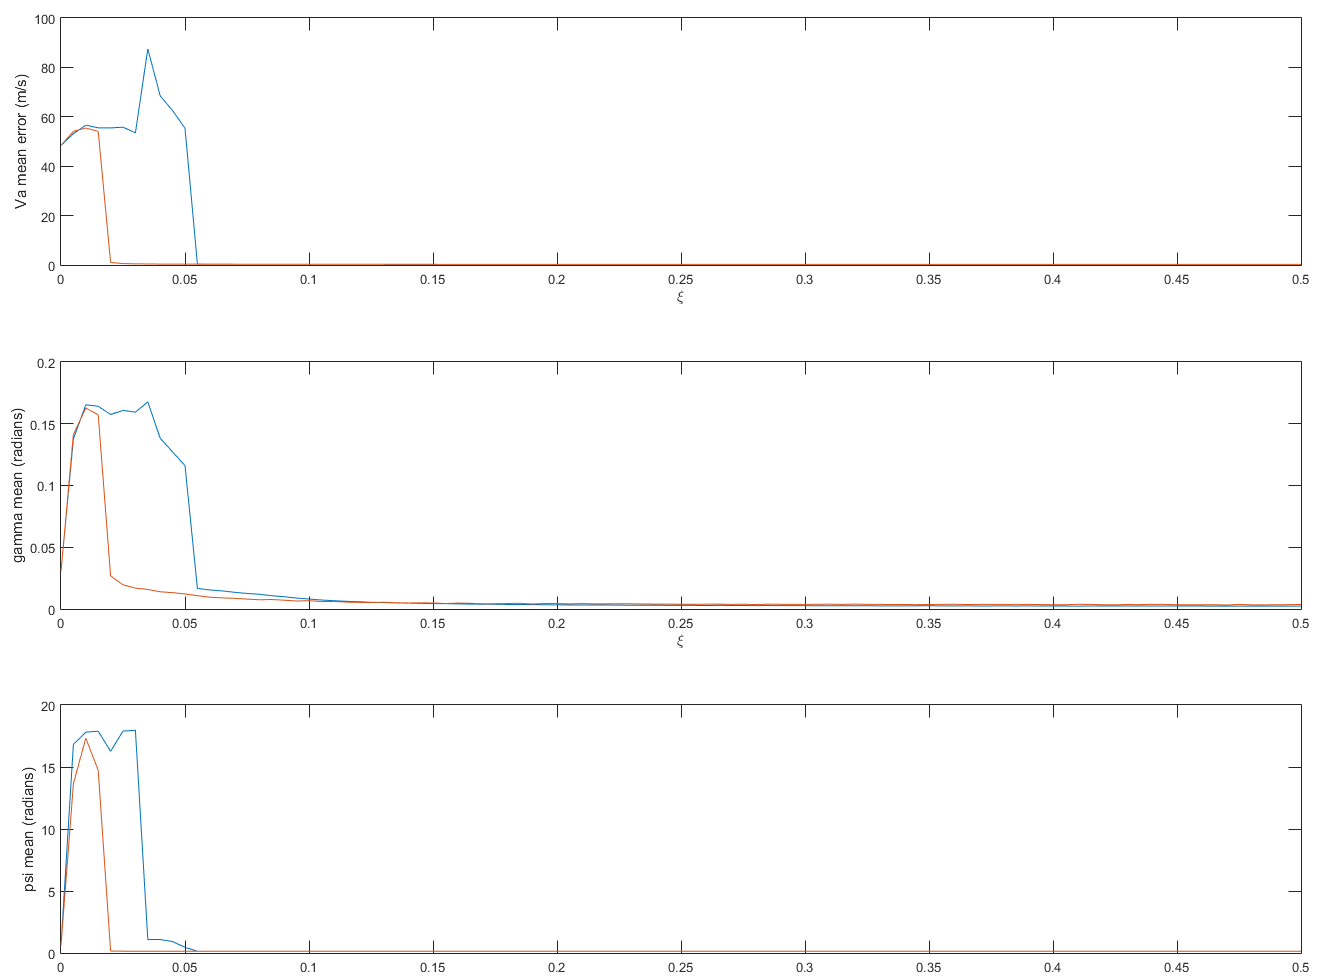
\includegraphics[width=0.5\textwidth]{../Figures/Results/mean_error_xi.png}
\caption[Mean errors for $V_a$, $\gamma$ and $psi$]{Mean errors for $V_a$, $\gamma$ and $psi$ for $\zeta=[0,0.5]$ with neural network compensation (orange) and without compensation (blue)}
\label{fig:xi_mean_error}
\end{figure}

\subsection{System Failures and External Disturbances}

One other cause for inversion errors that can have a much greater impact on flight trajectory are system failures. This subsection will focus on methods to simulate these failures and observe the behaviour of the airplane trajectory for these cases. The reference trajectory that will be used shall be the same as used previously. The first failure to be simulated will be a control surfaces failure, that will lead to reduced controllability of the aircraft. In this work this was replicated in a simulated environment by reducing by 80\% each moment coefficients for the elevator, aileron and rudder, namely $C_{\delta_{ele}}$, $C_{\delta_{ail}}$ and $C_{\delta_{rud}}$.

Applying the adaptive correction through the online neural network, the following trajectories were obtained

\begin{figure}[h]
\centering
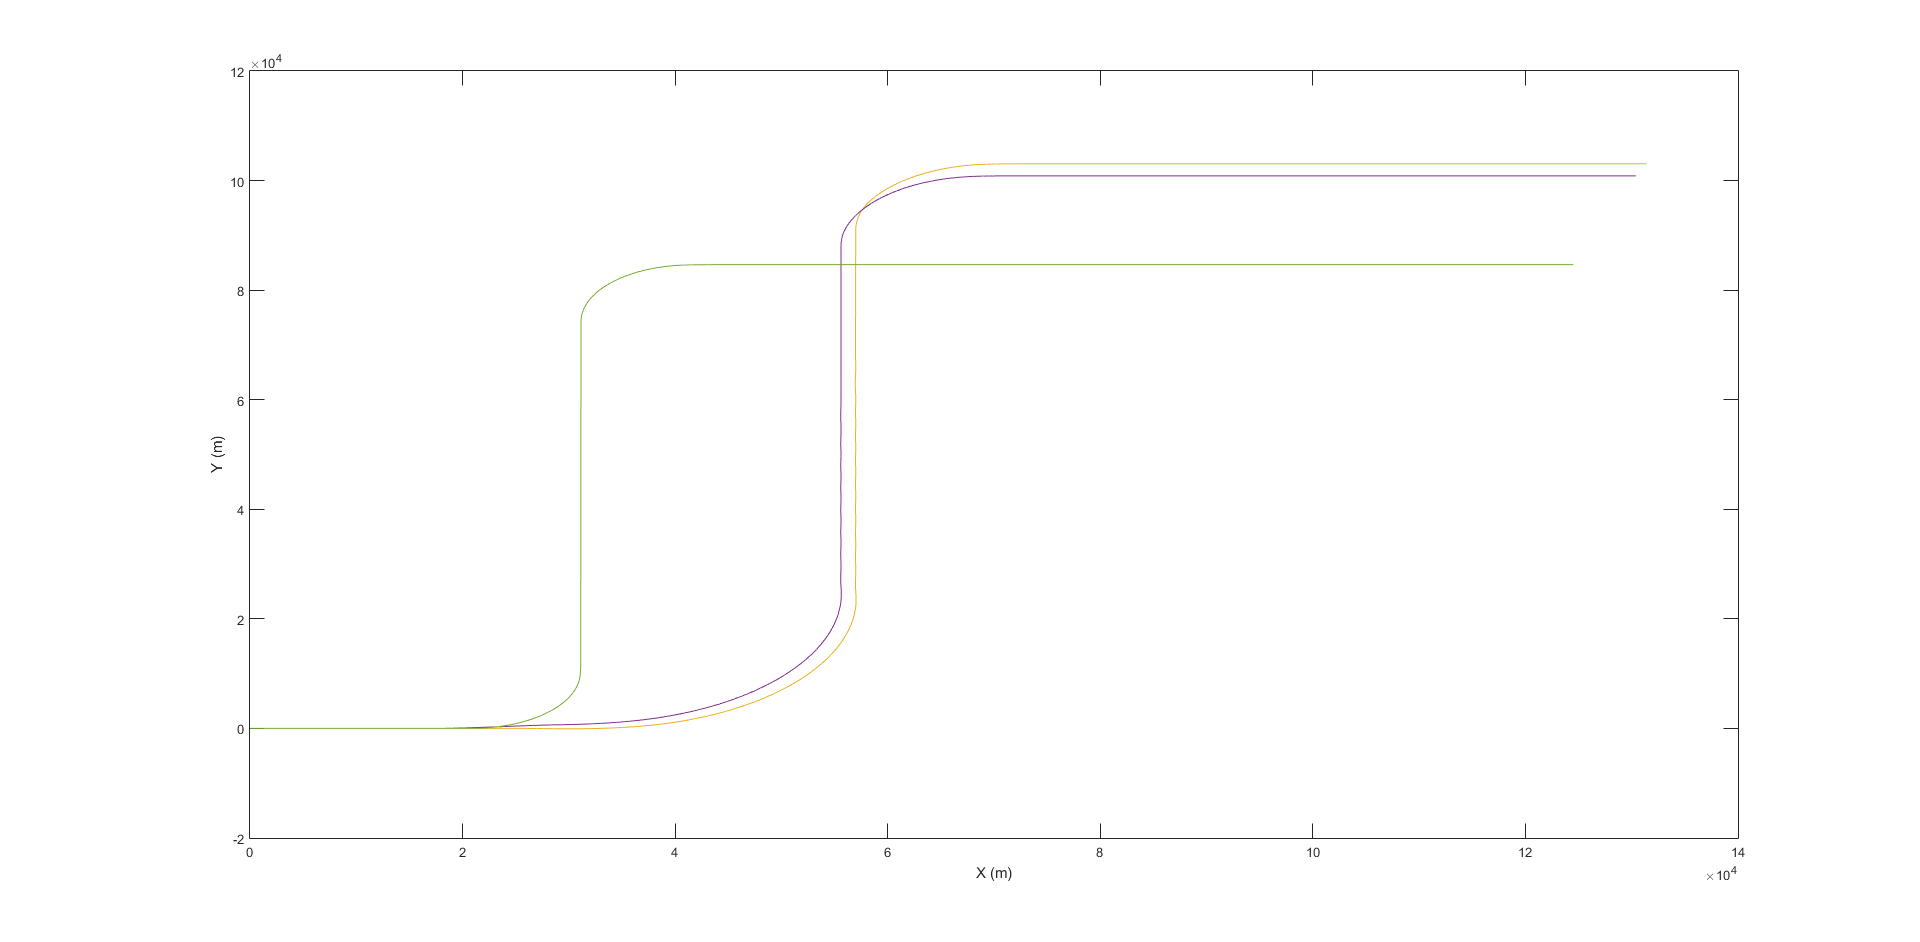
\includegraphics[width=0.5\textwidth]{../Figures/Results/reduced_act_NN.png}
\caption[Trajectory with reduced actuation corrected with NN correction]{Trajectory with 20\% reduced actuation (yellow) and trajectory without failures (green). The corrected trajectory by the NN can be seen in purple}
\label{fig:reduced_act_NN}
\end{figure}

The first observation that can be drawn from figure \ref{fig:reduced_act_NN} is that such an actuator failure severely reduces the controllability of the aircraft. 

The main consequence for this case will be, as could be expected, an increase in the convergence time to the desired heading. Note that the desired trajectory is not followed as this correction is only applied to the fast dynamics, and a guidance control law is not used. Comparing the two cases where the failures were implemented however, it can be observed that system corrected by the neural network converged to the desired heading slightly faster, resulting in a $2000m$ reduction in distance when comparing the non corrected control trajectory. 

